% Section 2: Decision Trees (Slides 7-18)

% Slide 7: Decision Tree Classifiers
\begin{frame}{طبقه‌بندهای درخت تصمیم}{\lr{Decision Tree Classifiers}}
  \begin{itemize}
    \item \textbf{تعریف:} درخت تصمیم ساختاری سلسله‌مراتبی است که یک رویه منسجم را برای اتخاذ تصمیم طبقه‌بندی کدگذاری می‌کند.
  \end{itemize}
  \vspace{0.2cm}
  \begin{center}
    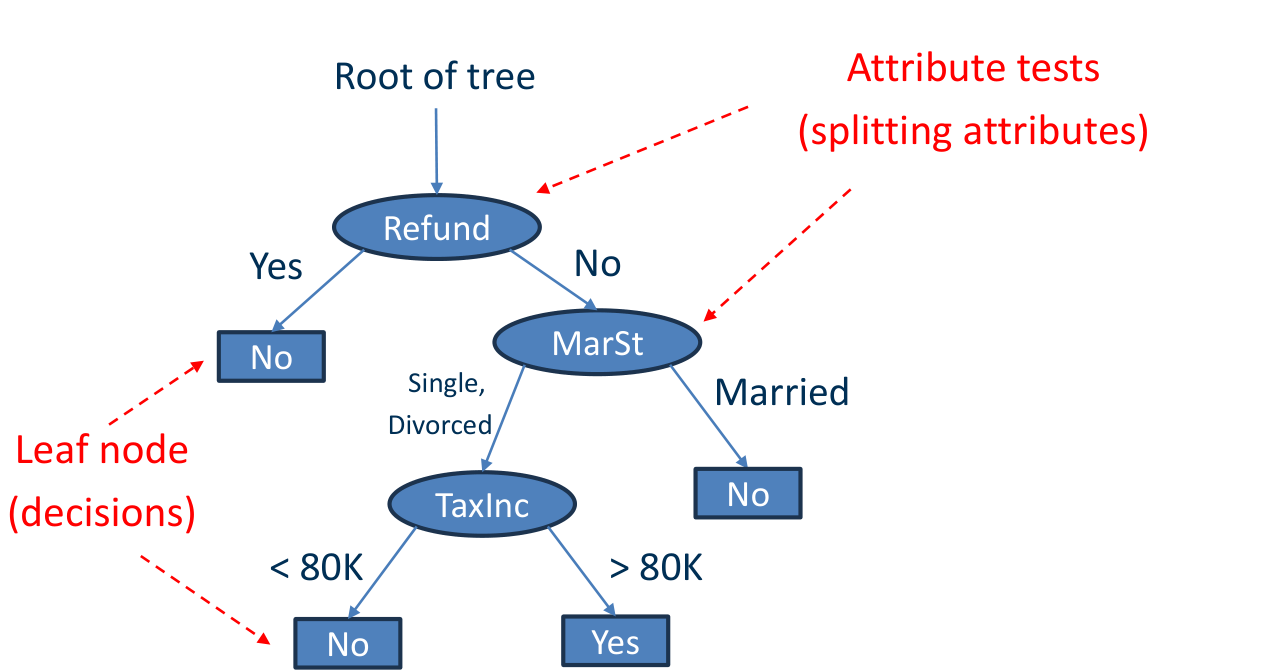
\includegraphics[width=0.90\textwidth,height=5.2cm,keepaspectratio]{images/slide07_tree_classifier_clean.png}
  \end{center}
\end{frame}

% Slide 8: Applying a Decision Tree to Unseen Data
\begin{frame}{اعمال درخت تصمیم بر داده‌های جدید}{مسیر ارزیابی یک رکورد نامشاهده‌شده}
  \begin{columns}[T]
    \begin{column}{0.48\textwidth}
      \begin{block}{رکورد نامشاهده‌شده (\lr{Unseen Record})}
        \centering\footnotesize
        \begin{tabular}{|c|c|c|c|}
          \hline
          \textbf{Refund} & \textbf{Marital} & \textbf{Taxable} & \textbf{Cheat} \\
          \hline
          No & Married & 80K & \textbf{?} \\
          \hline
        \end{tabular}
      \end{block}
      \vspace{0.2cm}
      \begin{itemize}
        \setlength{\itemsep}{6pt}
        \item \textbf{ردگیری گام‌به‌گام:}
        \begin{enumerate}
          \setlength{\itemsep}{3pt}
          \item آزمون ریشه (\lr{Refund}) -- مقدار برابر \codeinline{No} است $\to$ شاخه راست
          \item آزمون دوم (\lr{Marital}) -- وضعیت \codeinline{Married} است $\to$ شاخه چپ
          \item رسیدن به گره برگ: اختصاص برچسب \textbf{\lr{Cheat = "No"}}
        \end{enumerate}
      \end{itemize}
    \end{column}
    \begin{column}{0.50\textwidth}
      \begin{center}
        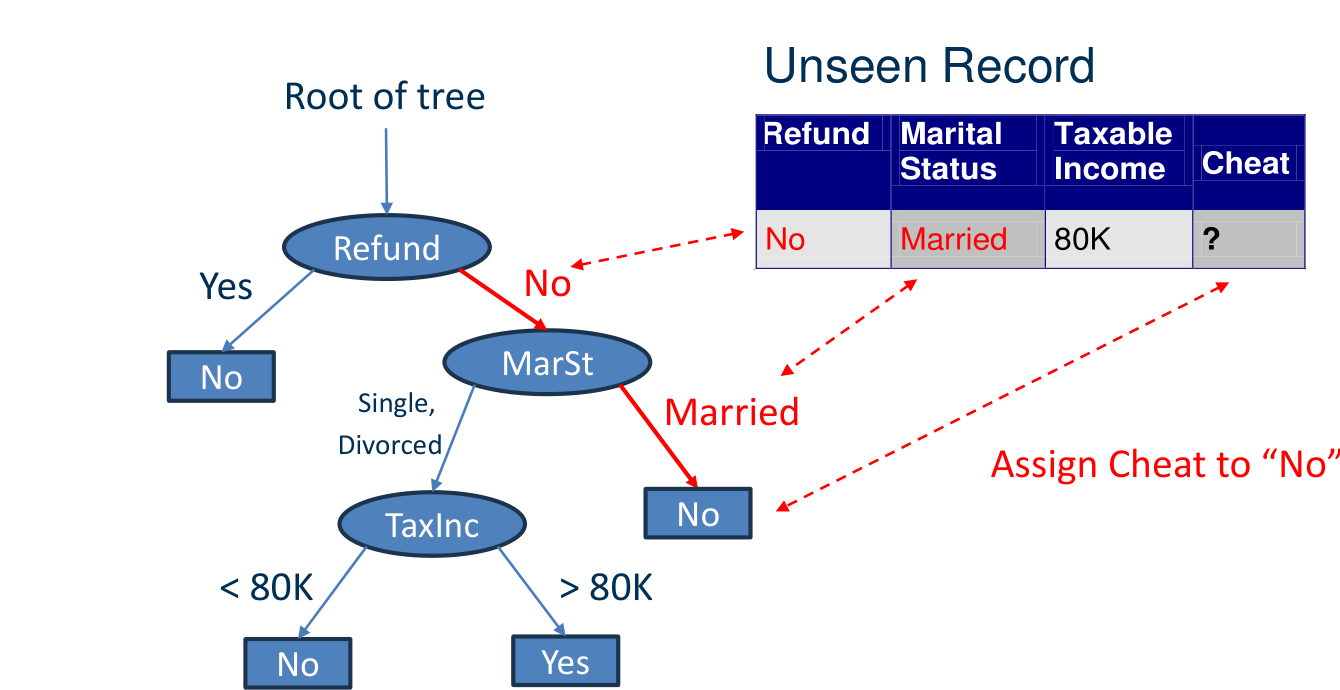
\includegraphics[width=\textwidth,height=5.2cm,keepaspectratio]{images/slide08_tree_unseen_clean.png}
      \end{center}
    \end{column}
  \end{columns}
\end{frame}

% Slide 9: Decision Boundary
\begin{frame}{مرزهای تصمیم در درخت تصمیم}{\lr{Decision Boundaries}}
  \begin{itemize}
    \item \textbf{تعامد با محورها:} مرزهای تصمیم در درخت‌های تصمیم همواره موازی با محورهای مختصات هستند (\lr{Axis-parallel})؛ زیرا هر شرط آزمون در هر مرحله تنها یک ویژگی را به تنهایی بررسی می‌کند.
  \end{itemize}
  \vspace{0.1cm}
  \begin{center}
    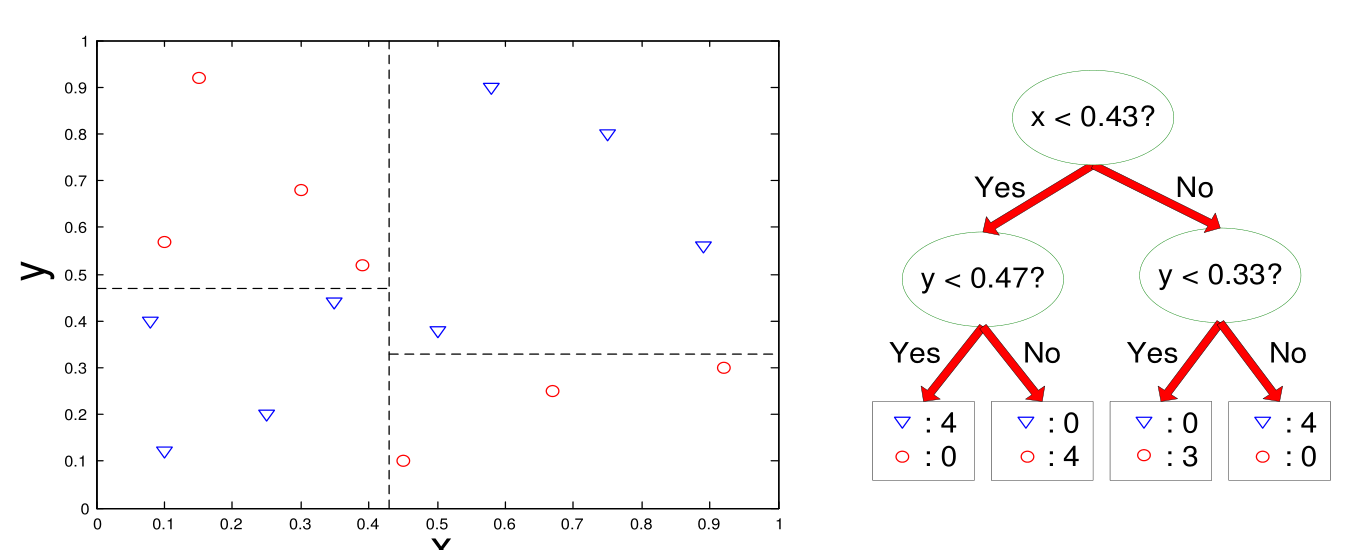
\includegraphics[width=0.90\textwidth,height=4.9cm,keepaspectratio]{images/slide09_decision_boundary_clean.png}
  \end{center}
\end{frame}

% Slide 10: Learning a Decision Tree
\begin{frame}{یادگیری و القای درخت تصمیم}{\lr{Learning a Decision Tree}}
  \begin{itemize}
    \setlength{\itemsep}{4pt}
    \item \textbf{چالش بهینه‌سازی:} یافتن درخت تصمیم بهینه سراسری از نظر محاسباتی یک مسئله \lr{NP-hard} است.
    \item \textbf{استراتژی تقسیم و حل:} \lr{(Divide and Conquer)} الگوریتم‌ها از یک رویکرد حریصانه (\lr{Greedy})، بالا به پایین (\lr{Top-down}) و افراز بازگشتی برای ساخت یک درخت منطقی استفاده می‌کنند.
  \end{itemize}
  \begin{columns}[c]
    \begin{column}{0.44\textwidth}
      \begin{itemize}
        \item \textbf{الگوریتم‌های ارائه‌شده:}
        \begin{itemize}\setlength{\itemsep}{2pt}
          \item الگوریتم هانت (\lr{Hunt's})
          \item الگوریتم \lr{ID3}
          \item الگوریتم \lr{C4.5}
          \item الگوریتم \lr{CHAID}
        \end{itemize}
      \end{itemize}
    \end{column}
    \begin{column}{0.54\textwidth}
      \begin{center}
        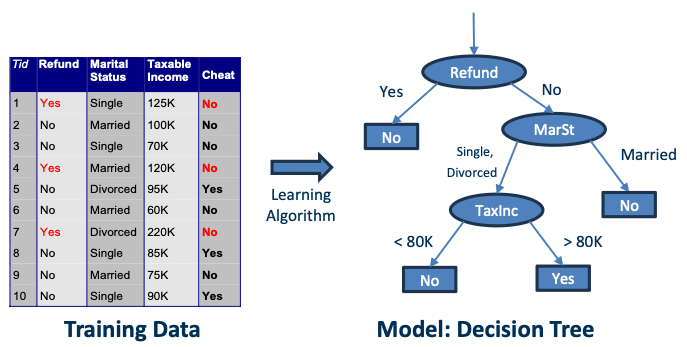
\includegraphics[width=\textwidth,height=3.8cm,keepaspectratio]{images/slide10_induction_workflow_clean.png}
      \end{center}
    \end{column}
  \end{columns}
\end{frame}

% Slide 11: Hunt's Algorithm
\begin{frame}{الگوریتم هانت}{\lr{Hunt's Algorithm}}
  \begin{columns}[c]
    \begin{column}{0.62\textwidth}
      \begin{itemize}
        \setlength{\itemsep}{5pt}
        \item فرض کنید $D_t$ مجموعه نمونه‌های آموزشی باشد که به گره $t$ می‌رسند.
        \item \textbf{تولید گره برگ یا آزمون ویژگی:}
        \begin{itemize}
          \setlength{\itemsep}{2pt}
          \item اگر تمام رکوردهای $D_t$ به یک کلاس واحد $y_t$ تعلق داشته باشند، آنگاه $t$ یک \textbf{گره برگ} با برچسب $y_t$ خواهد بود.
          \item اگر $D_t$ شامل رکوردهایی از بیش از یک کلاس باشد، از یک \textbf{آزمون ویژگی} برای تفکیک داده‌ها به زیرمجموعه‌های با خلوص بالاتر استفاده می‌شود.
        \end{itemize}
        \item \textbf{انتخاب آزمون بهینه:} برای تمام آزمون‌های ممکن، خلوص محاسبه شده و آزمونی که خالص‌ترین افراز را بدهد برگزیده می‌شود.
        \item این رویه به صورت \textbf{بازگشتی} بر روی هر زیرمجموعه اعمال می‌شود.
      \end{itemize}
    \end{column}
    \begin{column}{0.36\textwidth}
      \begin{center}
        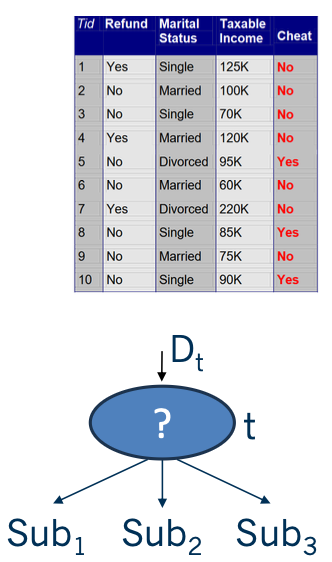
\includegraphics[width=\textwidth,height=5.8cm,keepaspectratio]{images/slide11_hunt_diagram_clean.png}
      \end{center}
    \end{column}
  \end{columns}
\end{frame}

% Slide 12: Hunt's Algorithm - Step 1
\begin{frame}{الگوریتم هانت -- گام ۱}{انتخاب اولین تفکیک خلوص}
  \begin{columns}[T]
    \begin{column}{0.50\textwidth}
      \begin{itemize}
        \setlength{\itemsep}{6pt}
        \item \textbf{محاسبه خلوص زیرمجموعه‌ها} برای تمام ویژگی‌ها:
        \begin{itemize}
          \item خلوص تفکیک روی بازپرداخت (\lr{Refund})
          \item خلوص تفکیک روی وضعیت تأهل (\lr{Marital Status})
          \item خلوص تفکیک روی درآمد مشمول مالیات (\lr{Taxable Income})
        \end{itemize}
        \item \textbf{نتیجه:} تفکیک بر اساس ویژگی \lr{Refund} خالص‌ترین زیرمجموعه‌ها را ایجاد می‌کند.
      \end{itemize}
    \end{column}
    \begin{column}{0.48\textwidth}
      \begin{center}
        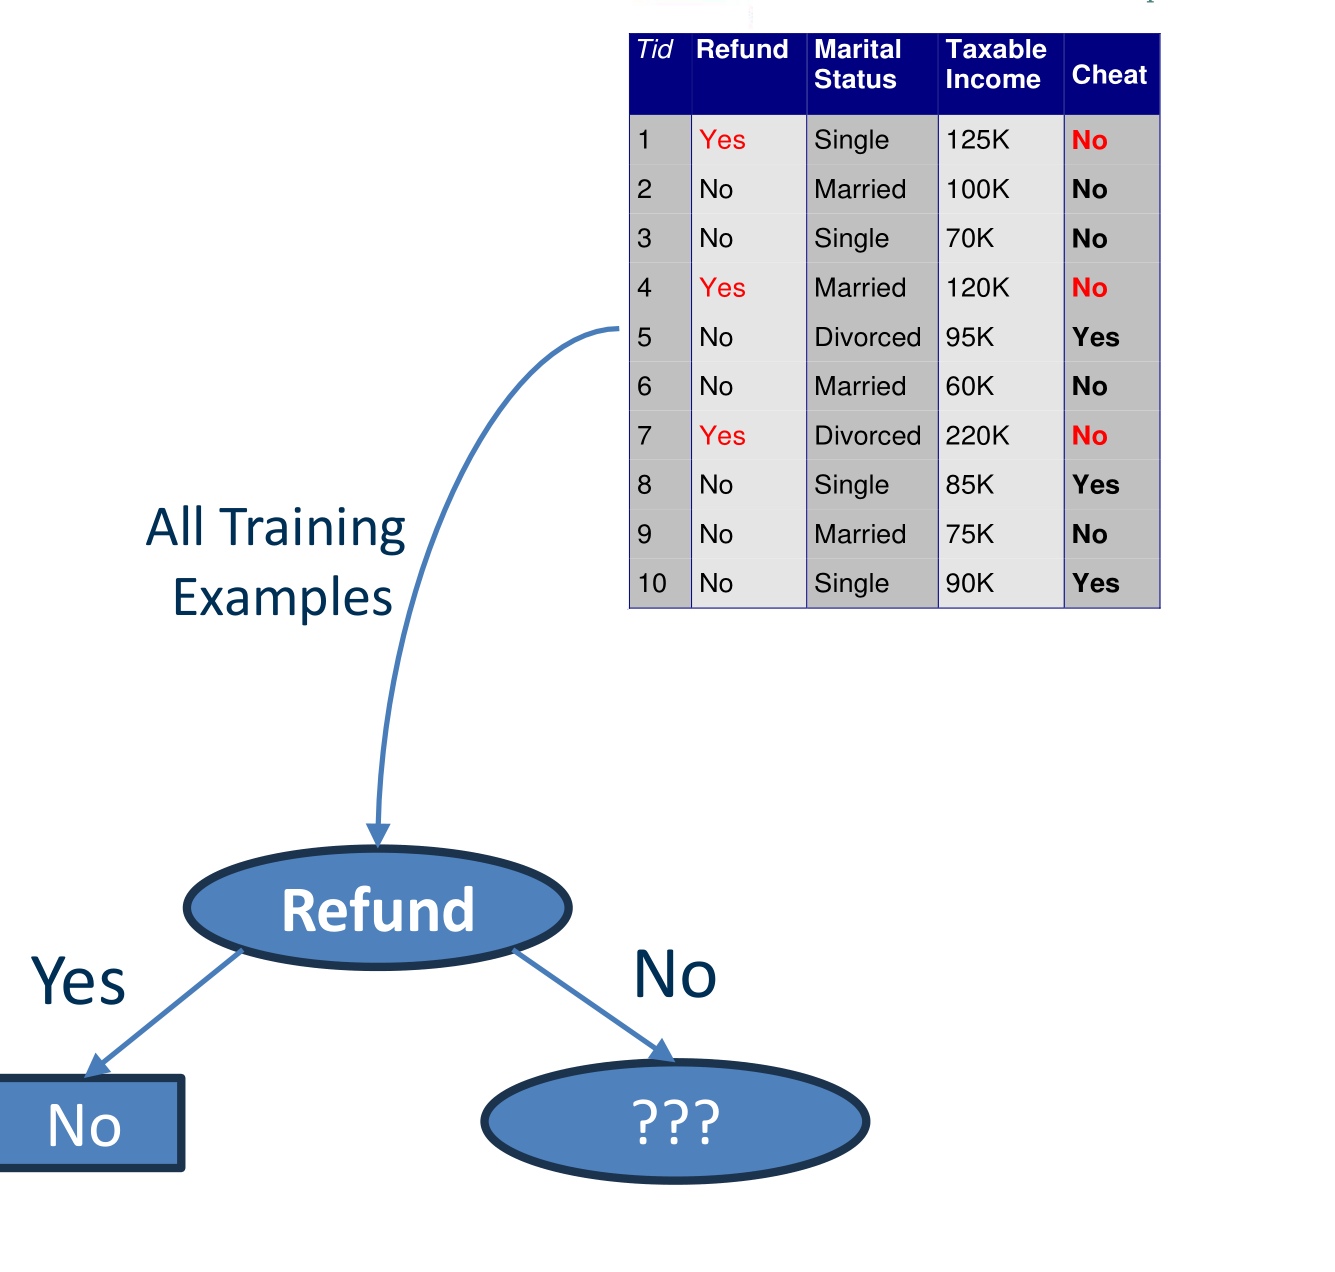
\includegraphics[width=\textwidth,height=4.8cm,keepaspectratio]{images/slide12_hunt_step1_composite.png}
      \end{center}
    \end{column}
  \end{columns}
\end{frame}

% Slide 13: Hunt's Algorithm - Step 2
\begin{frame}{الگوریتم هانت -- گام ۲}{تفکیک رکوردهای شاخه \lr{Refund = No}}
  \begin{columns}[T]
    \begin{column}{0.50\textwidth}
      \begin{itemize}
        \setlength{\itemsep}{6pt}
        \item بررسی ۷ رکورد با شرط \codeinline{Refund = No}
        \item آزمون مجدد ویژگی‌های باقیمانده بر روی این زیرمجموعه
        \item \textbf{نتیجه:} تفکیک بر اساس وضعیت تأهل (\lr{Marital Status}) بالاترین خلوص را دارد
        \begin{itemize}
          \item افراد متأهل (\lr{Married}) همه \lr{Cheat = No} (برگ خالص)
          \item مجرد و طلاق‌گرفته: نامتعادل (نیازمند انشعاب بیشتر)
        \end{itemize}
      \end{itemize}
    \end{column}
    \begin{column}{0.48\textwidth}
      \begin{center}
        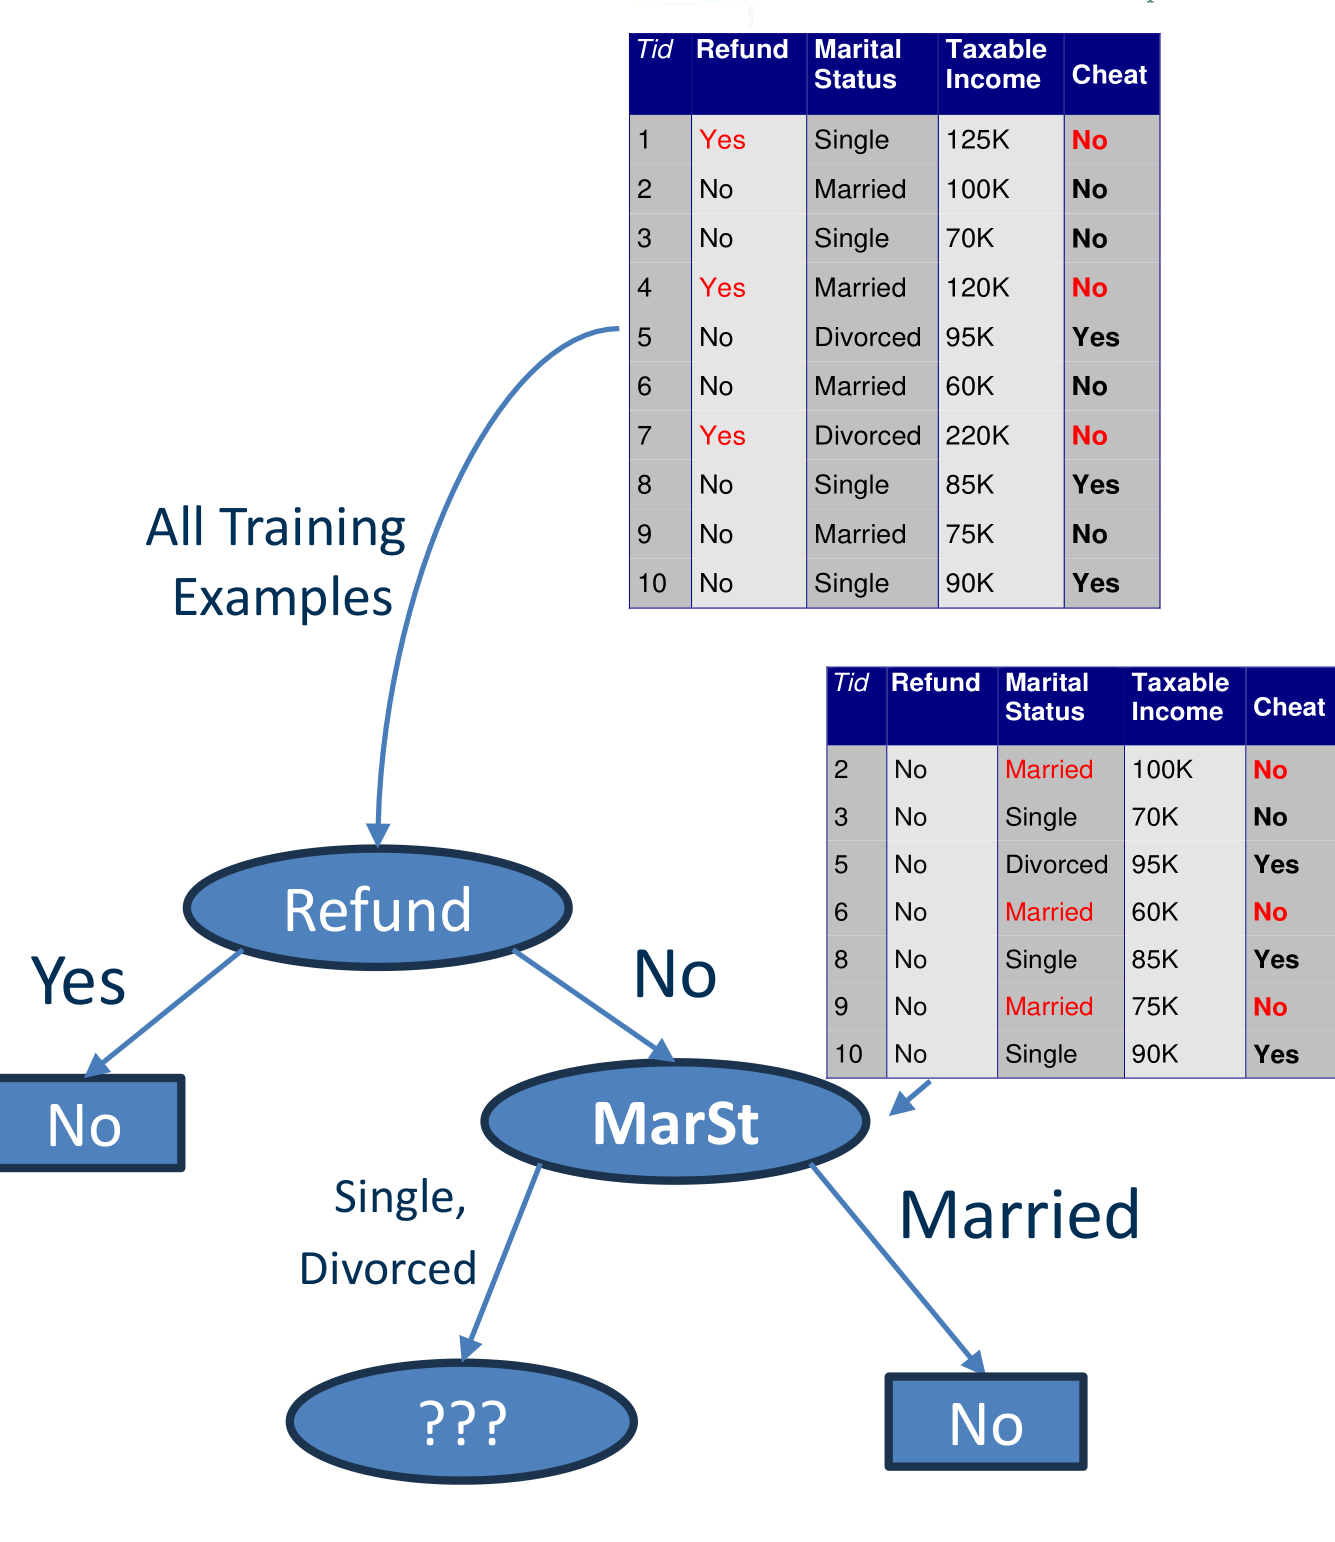
\includegraphics[width=\textwidth,height=4.9cm,keepaspectratio]{images/slide13_hunt_step2_composite.png}
      \end{center}
    \end{column}
  \end{columns}
\end{frame}

% Slide 14: Hunt's Algorithm - Step 3
\begin{frame}{الگوریتم هانت -- گام ۳}{تکمیل درخت و خالص‌سازی تمامی برگ‌ها}
  \begin{columns}[T]
    \begin{column}{0.48\textwidth}
      \begin{itemize}
        \setlength{\itemsep}{5pt}
        \item بررسی رکوردهای زیرمجموعه \lr{Single / Divorced} (۴ رکورد)
        \item تفکیک روی درآمد مشمول مالیات (\lr{Taxable Income})
        \begin{itemize}
          \item $\text{Income} < 80\text{K} \implies \text{Cheat} = \text{No}$
          \item $\text{Income} \ge 80\text{K} \implies \text{Cheat} = \text{Yes}$
        \end{itemize}
        \item \textbf{شرط توقف:} تمام گره‌ها خالص شده و الگوریتم خاتمه می‌یابد.
      \end{itemize}
    \end{column}
    \begin{column}{0.50\textwidth}
      \begin{center}
        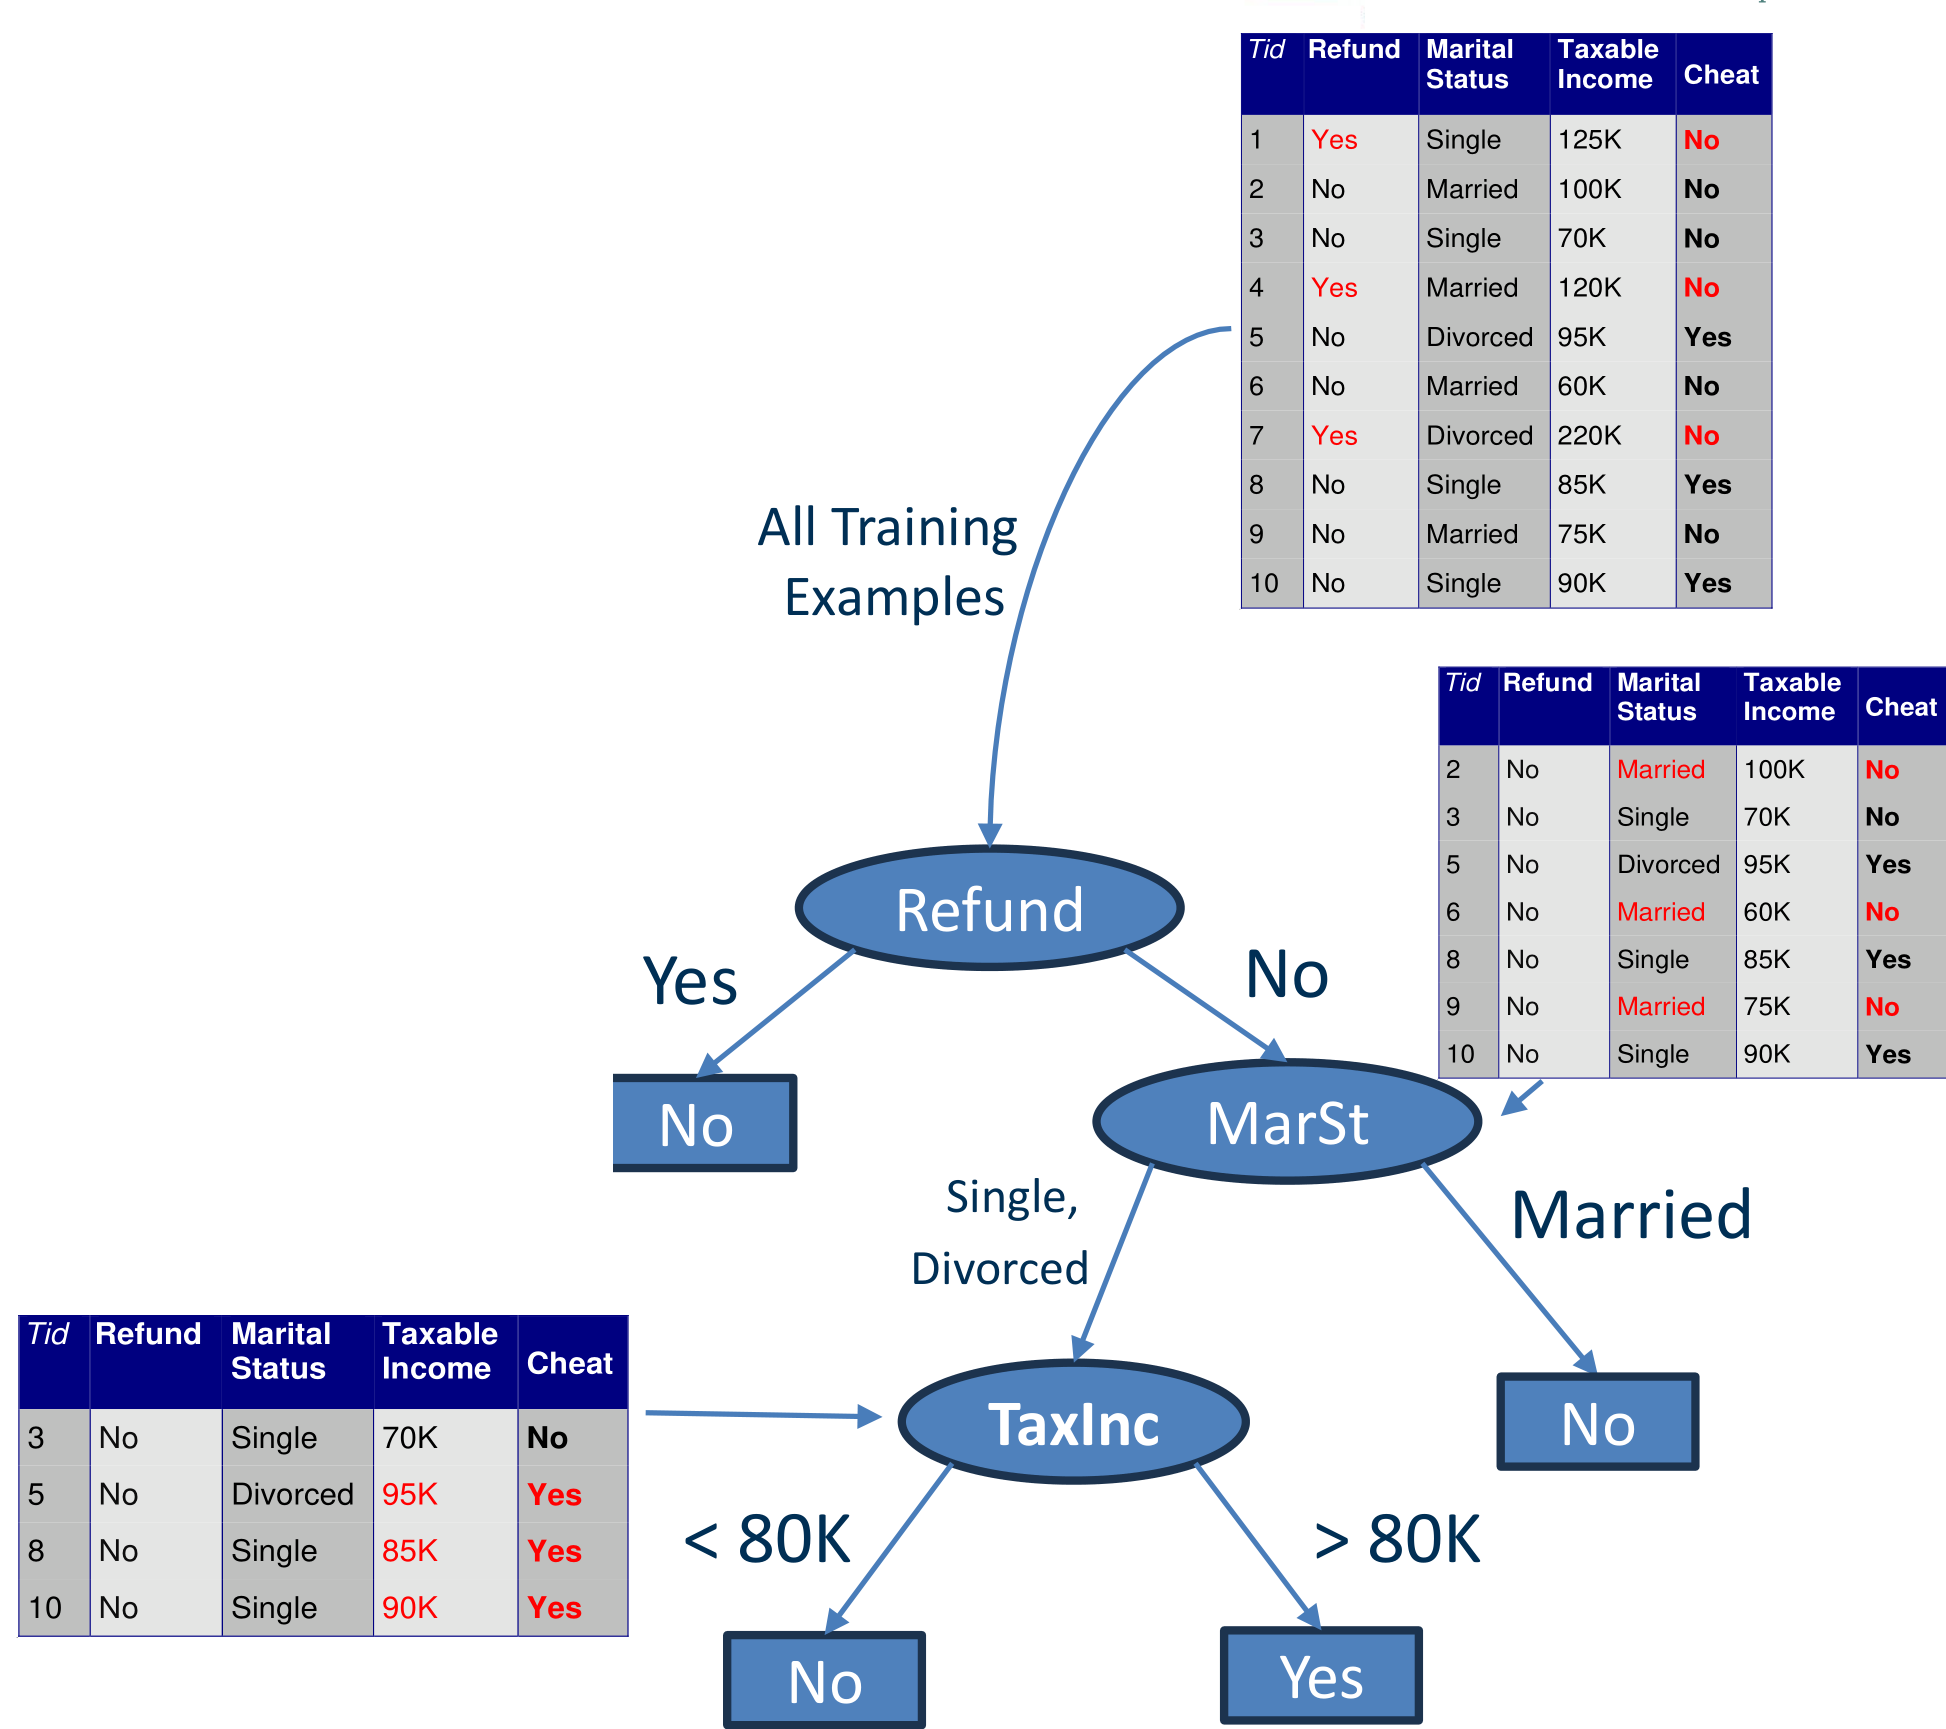
\includegraphics[width=\textwidth,height=5.0cm,keepaspectratio]{images/slide14_hunt_step3_composite.png}
      \end{center}
    \end{column}
  \end{columns}
\end{frame}

% Slide 15: Tree Induction Issues
\begin{frame}{چالش‌های کلیدی در القای درخت تصمیم}{\lr{Tree Induction Issues}}
  \begin{itemize}
    \setlength{\itemsep}{12pt}
    \item \textbf{مسئله اول: چگونگی تفکیک نمونه‌ها (\lr{How to split records?})}
    \begin{itemize}
      \setlength{\itemsep}{4pt}
      \item نحوه تعریف شرایط آزمون برای انواع ویژگی‌ها:
      \begin{itemize}
        \item ویژگی‌های اسمی (\lr{Nominal})
        \item ویژگی‌های ترتیبی (\lr{Ordinal})
        \item ویژگی‌های عددی و پیوسته (\lr{Continuous})
      \end{itemize}
      \item انتخاب بهترین شرط تفکیک از میان گزینه‌های کاندید (معیارهای ناخالصی)
    \end{itemize}
    \item \textbf{مسئله دوم: چگونگی توقف الگوریتم (\lr{Stopping condition})}
    \begin{itemize}
      \setlength{\itemsep}{4pt}
      \item توقف زمانی که تمامی نمونه‌های یک گره به کلاس یکسانی تعلق داشته باشند.
      \item توقف زمانی که مقادیر تمام ویژگی‌ها برای نمونه‌های باقیمانده یکسان باشد.
      \item توقف زودهنگام (\lr{Early Stopping}) جهت مقابله با بیش‌برازش.
    \end{itemize}
  \end{itemize}
\end{frame}

% Slide 16: Splitting Nominal Attributes
\begin{frame}{تفکیک ویژگی‌های اسمی}{\lr{Splitting of Nominal Attributes}}
  \begin{itemize}\setlength{\itemsep}{1pt}
    \item \textbf{تفکیک چندگانه (\lr{Multi-way split}):} ایجاد به تعداد مقادیر مجزای ویژگی:
    \begin{center}
      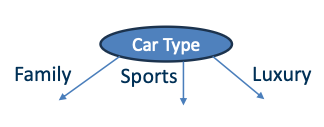
\includegraphics[width=0.36\textwidth,height=1.4cm,keepaspectratio]{images/slide16_car_multiway_clean.png}
    \end{center}
    \item \textbf{تفکیک دوتایی (\lr{Binary split}):} افراز به دو زیرمجموعه با $2^{k-1}-1$ حالت ممکن:
    \begin{center}
      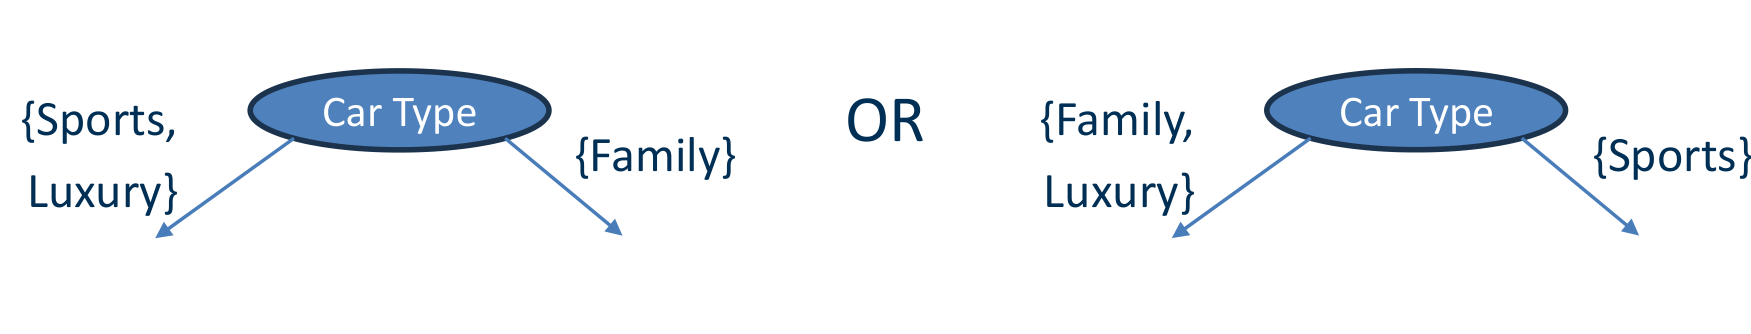
\includegraphics[width=0.82\textwidth,height=2.0cm,keepaspectratio]{images/slide16_car_binary_clean.png}
    \end{center}
  \end{itemize}
\end{frame}

% Slide 17: Splitting Ordinal Attributes
\begin{frame}{تفکیک ویژگی‌های ترتیبی}{\lr{Splitting of Ordinal Attributes}}
  \begin{itemize}\setlength{\itemsep}{1pt}
    \item \textbf{تفکیک چندگانه (\lr{Multi-way split}):} ایجاد به تعداد مقادیر مجزا:
    \begin{center}
      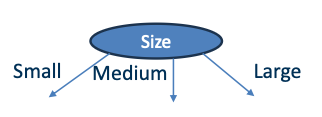
\includegraphics[width=0.36\textwidth,height=1.4cm,keepaspectratio]{images/slide17_size_multiway_clean.png}
    \end{center}
    \item \textbf{تفکیک دوتایی (\lr{Binary split}):} افراز به دو زیرمجموعه \textbf{با حفظ ترتیب مقادیر}:
    \begin{center}
      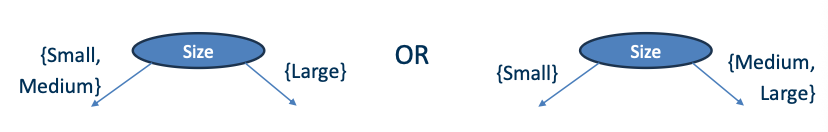
\includegraphics[width=0.85\textwidth,height=1.9cm,keepaspectratio]{images/slide17_size_binary_clean.png}
    \end{center}
  \end{itemize}
\end{frame}

% Slide 18: Splitting Continuous Attributes
\begin{frame}{تفکیک ویژگی‌های عددی و پیوسته}{\lr{Splitting of Continuous Attributes}}
  \begin{columns}[c]
    \begin{column}{0.54\textwidth}
      \begin{itemize}
        \setlength{\itemsep}{6pt}
        \item \textbf{تفکیک چندگانه با گسسته‌سازی:} \lr{(Discretization)}
        \begin{itemize}\setlength{\itemsep}{2pt}
          \item تبدیل مقادیر پیوسته به بازه‌های ترتیبی (مانند $[10, 25)$، $[25, 50)$، $[50, 80)$)
          \item رویکردهای فاصله‌های ایستا یا تطبیقی
        \end{itemize}
        \item \textbf{تفکیک دوتایی:} \lr{(Binary Decision)}
        \begin{itemize}\setlength{\itemsep}{2pt}
          \item انتخاب یک آستانه بهینه $v$ به شکل آزمون $A < v$ در برابر $A \ge v$
          \item بررسی تمام مقادیر میانی کاندید برای بیشینه‌سازی خلوص
        \end{itemize}
      \end{itemize}
    \end{column}
    \begin{column}{0.44\textwidth}
      \begin{center}
        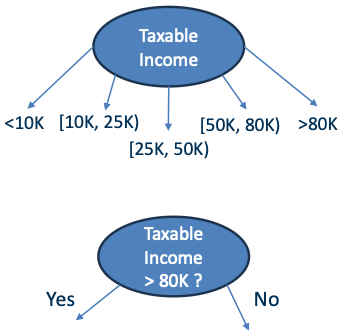
\includegraphics[width=\textwidth,height=5.2cm,keepaspectratio]{images/slide18_continuous_splits_clean.png}
      \end{center}
    \end{column}
  \end{columns}
\end{frame}
